%%%%%%%%%%%%%%%%%%%%%%%%%%%%%%%%%%%%%%%%%
% Masters/Doctoral Thesis 
% LaTeX Template
% Version 2.5 (27/8/17)
% Template license:
% CC BY-NC-SA 3.0 (http://creativecommons.org/licenses/by-nc-sa/3.0/)
%
%%%%%%%%%%%%%%%%%%%%%%%%%%%%%%%%%%%%%%%%%

%----------------------------------------------------------------------------------------
%	PACKAGES AND OTHER DOCUMENT CONFIGURATIONS
%----------------------------------------------------------------------------------------

\documentclass[
11pt, % The default document font size, options: 10pt, 11pt, 12pt
%oneside, % Two side (alternating margins) for binding by default, uncomment to switch to one side
english, % ngerman for German
singlespacing, % Single line spacing, alternatives: onehalfspacing or doublespacing
%draft, % Uncomment to enable draft mode (no pictures, no links, overfull hboxes indicated)
%nolistspacing, % If the document is onehalfspacing or doublespacing, uncomment this to set spacing in lists to single
%liststotoc, % Uncomment to add the list of figures/tables/etc to the table of contents
%toctotoc, % Uncomment to add the main table of contents to the table of contents
%parskip, % Uncomment to add space between paragraphs
%nohyperref, % Uncomment to not load the hyperref package
headsepline, % Uncomment to get a line under the header
%chapterinoneline, % Uncomment to place the chapter title next to the number on one line
%consistentlayout, % Uncomment to change the layout of the declaration, abstract and acknowledgements pages to match the default layout
tikz,
oneside,
]{MastersDoctoralThesis} % The class file specifying the document structure

\usepackage[utf8]{inputenc} % Required for inputting international characters
\usepackage[T1]{fontenc} % Output font encoding for international characters

\usepackage{mathpazo} % Use the Palatino font by default
\usepackage{tikz}
\usetikzlibrary{arrows, chains, fit, quotes}

\usepackage[backend=bibtex,style=authoryear,natbib=true]{biblatex} % Use the bibtex backend with the authoryear citation style (which resembles APA)

\usepackage[demo]{graphicx}
\usepackage{subcaption}
\usepackage{minted}

\addbibresource{example.bib} % The filename of the bibliography

\usepackage[autostyle=true]{csquotes} % Required to generate language-dependent quotes in the bibliography

%----------------------------------------------------------------------------------------
%	MARGIN SETTINGS
%----------------------------------------------------------------------------------------

\geometry{
	paper=a4paper, % Change to letterpaper for US letter
	inner=2.5cm, % Inner margin
	outer=3.8cm, % Outer margin
	bindingoffset=.5cm, % Binding offset
	top=1.5cm, % Top margin
	bottom=1.5cm, % Bottom margin
	%showframe, % Uncomment to show how the type block is set on the page
}

%----------------------------------------------------------------------------------------
%	THESIS INFORMATION
%----------------------------------------------------------------------------------------

\thesistitle{Source Accountability with Domain-brokered Privacy in SCION} % Your thesis title, this is used in the title and abstract, print it elsewhere with \ttitle
\supervisor{Dr. \textsc{Adrian} \textsc{Perrig}\\ Dr. \textsc{Taheo} \textsc{Lee}} % Your supervisor's name, this is used in the title page, print it elsewhere with \supname
\examiner{} % Your examiner's name, this is not currently used anywhere in the template, print it elsewhere with \examname
\degree{Masters of Science} % Your degree name, this is used in the title page and abstract, print it elsewhere with \degreename
\author{\textsc{Jinank} \textsc{Jain}} % Your name, this is used in the title page and abstract, print it elsewhere with \authorname
\addresses{} % Your address, this is not currently used anywhere in the template, print it elsewhere with \addressname

\subject{Network Security} % Your subject area, this is not currently used anywhere in the template, print it elsewhere with \subjectname
\keywords{} % Keywords for your thesis, this is not currently used anywhere in the template, print it elsewhere with \keywordnames
\university{\href{https://www.ethz.ch/}{ETH Z\"urich}} % Your university's name and URL, this is used in the title page and abstract, print it elsewhere with \univname
\department{\href{https://www.inf.ethz.ch/}{Department of Computer Science}} % Your department's name and URL, this is used in the title page and abstract, print it elsewhere with \deptname
\group{\href{http://www.netsec.ethz.ch/}{Network Security Group}} % Your research group's name and URL, this is used in the title page, print it elsewhere with \groupname
\faculty{\href{http://www.netsec.ethz.ch/people/aperrig/}{Dr. Adrian Perrig}} % Your faculty's name and URL, this is used in the title page and abstract, print it elsewhere with \facname

\AtBeginDocument{
\hypersetup{pdftitle=\ttitle} % Set the PDF's title to your title
\hypersetup{pdfauthor=\authorname} % Set the PDF's author to your name
\hypersetup{pdfkeywords=\keywordnames} % Set the PDF's keywords to your keywords
}

\begin{document}

\frontmatter % Use roman page numbering style (i, ii, iii, iv...) for the pre-content pages

\pagestyle{plain} % Default to the plain heading style until the thesis style is called for the body content

%----------------------------------------------------------------------------------------
%	TITLE PAGE
%----------------------------------------------------------------------------------------

\begin{titlepage}
\begin{center}

\vspace*{.06\textheight}
{\scshape\LARGE \univname\par}\vspace{1.5cm} % University name
\textsc{\Large Master's Thesis}\\[0.5cm] % Thesis type

\HRule \\[0.4cm] % Horizontal line
{\huge \bfseries \ttitle\par}\vspace{0.4cm} % Thesis title
\HRule \\[1.5cm] % Horizontal line
 
\begin{minipage}[t]{0.4\textwidth}
\begin{flushleft} \large
\emph{Author:}\\
\href{http://www.jinankjain.com}{\authorname} % Author name - remove the \href bracket to remove the link
\end{flushleft}
\end{minipage}
\begin{minipage}[t]{0.4\textwidth}
\begin{flushright} \large
\emph{Supervisor:} \\
\href{http://www.netsec.ethz.ch/people/aperrig/}{\supname} % Supervisor name - remove the \href bracket to remove the link  
\end{flushright}
\end{minipage}\\[3cm]
 
\vfill

\large \textit{A thesis submitted in partial fulfillment of the requirements\\ for the degree of \degreename}\\[0.3cm] % University requirement text
\textit{in the}\\[0.4cm]
\groupname\\\deptname\\[2cm] % Research group name and department name
 
\vfill

{\large \today}\\[4cm] % Date
%\includegraphics{Logo} % University/department logo - uncomment to place it
 
\vfill
\end{center}
\end{titlepage}

%----------------------------------------------------------------------------------------
%	DECLARATION PAGE
%----------------------------------------------------------------------------------------

\begin{declaration}
\addchaptertocentry{\authorshipname} % Add the declaration to the table of contents
\noindent I, \authorname, declare that this thesis titled, \enquote{\ttitle} and the work presented in it are my own. I confirm that:

\begin{itemize} 
\item This work was done wholly or mainly while in candidature for a research degree at this University.
\item Where any part of this thesis has previously been submitted for a degree or any other qualification at this University or any other institution, this has been clearly stated.
\item Where I have consulted the published work of others, this is always clearly attributed.
\item Where I have quoted from the work of others, the source is always given. With the exception of such quotations, this thesis is entirely my own work.
\item I have acknowledged all main sources of help.
\item Where the thesis is based on work done by myself jointly with others, I have made clear exactly what was done by others and what I have contributed myself.\\
\end{itemize}
 
\noindent Signed:\\
\rule[0.5em]{25em}{0.5pt} % This prints a line for the signature
 
\noindent Date:\\
\rule[0.5em]{25em}{0.5pt} % This prints a line to write the date
\end{declaration}

\cleardoublepage

%----------------------------------------------------------------------------------------
%	QUOTATION PAGE
%----------------------------------------------------------------------------------------

\vspace*{0.2\textheight}

\noindent\enquote{\itshape Thanks to my solid academic training, today I can write hundreds of words on virtually any topic without possessing a shred of information, which is how I got a good job in journalism.}\bigbreak

\hfill Jinank Jain

%----------------------------------------------------------------------------------------
%	ABSTRACT PAGE
%----------------------------------------------------------------------------------------

\begin{abstract}
\addchaptertocentry{\abstractname} % Add the abstract to the table of contents
The Thesis Abstract is written here (and usually kept to just this page). The page is kept centered vertically so can expand into the blank space above the title too\ldots
\end{abstract}

%----------------------------------------------------------------------------------------
%	ACKNOWLEDGEMENTS
%----------------------------------------------------------------------------------------

\begin{acknowledgements}
\addchaptertocentry{\acknowledgementname} % Add the acknowledgements to the table of contents
The acknowledgments and the people to thank go here, don't forget to include your project advisor\ldots
\end{acknowledgements}

%----------------------------------------------------------------------------------------
%	LIST OF CONTENTS/FIGURES/TABLES PAGES
%----------------------------------------------------------------------------------------

\tableofcontents % Prints the main table of contents

\listoffigures % Prints the list of figures

\listoftables % Prints the list of tables

%----------------------------------------------------------------------------------------
%	ABBREVIATIONS
%----------------------------------------------------------------------------------------

\begin{abbreviations}{ll} % Include a list of abbreviations (a table of two columns)

\textbf{APNA} & \textbf{A}ccountable \textbf{P}rivate \textbf{N}etwork \textbf{A}rchitecture \\
\textbf{DNS} & \textbf{D}omain \textbf{N}ame \textbf{S}ystem \\
\textbf{IP} & \textbf{I}nternet \textbf{P}rotocol \\
\textbf{SCION} & \textbf{S}calability \textbf{C}ontrol \textbf{I}solation \textbf{O}n Next-Generation \textbf{N}etworks \\
\textbf{BR} & \textbf{B}order \textbf{R}outer \\
\textbf{ISD} & \textbf{IS}olation \textbf{D}omain \\
\textbf{AS} & \textbf{A}utonomous \textbf{S}ystem \\

\end{abbreviations}

%----------------------------------------------------------------------------------------
%	PHYSICAL CONSTANTS/OTHER DEFINITIONS
%----------------------------------------------------------------------------------------

% \begin{constants}{lr@{${}={}$}l} % The list of physical constants is a three column table

% % The \SI{}{} command is provided by the siunitx package, see its documentation for instructions on how to use it

% Speed of Light & $c_{0}$ & \SI{2.99792458e8}{\meter\per\second} (exact)\\
% %Constant Name & $Symbol$ & $Constant Value$ with units\\

% \end{constants}

% %----------------------------------------------------------------------------------------
% %	SYMBOLS
% %----------------------------------------------------------------------------------------

% \begin{symbols}{lll} % Include a list of Symbols (a three column table)

% $a$ & distance & \si{\meter} \\
% $P$ & power & \si{\watt} (\si{\joule\per\second}) \\
% %Symbol & Name & Unit \\

% \addlinespace % Gap to separate the Roman symbols from the Greek

% $\omega$ & angular frequency & \si{\radian} \\

% \end{symbols}

%----------------------------------------------------------------------------------------
%	DEDICATION
%----------------------------------------------------------------------------------------

\dedicatory{For/Dedicated to/To my\ldots} 

%----------------------------------------------------------------------------------------
%	THESIS CONTENT - CHAPTERS
%----------------------------------------------------------------------------------------

\mainmatter % Begin numeric (1,2,3...) page numbering

\pagestyle{thesis} % Return the page headers back to the "thesis" style

% Include the chapters of the thesis as separate files from the Chapters folder
% Uncomment the lines as you write the chapters

% Chapter Introduction

\chapter{Introduction} % Main chapter title

\label{intro} % For referencing the chapter elsewhere, use \ref{intro}

% Chapter Background

\chapter{Background} % Main chapter title

\label{background} % For referencing the chapter elsewhere, use \ref{background}

\section{What is SCION?}
SCION is the new clean state internet architecture designed to provide explicit route control, failure isolation, and explicit trust information for end-to-end communication. SCION organizes existing ASes into groups of independent routing planes, called isolation domains, which interconnect to provide global connectivity. Isolation domains provide natural isolation of routing failures and misconfigurations, give endpoints strong control for both inbound and outbound traffic, provide meaningful and enforceable trust, and enable scalable routing updates with high path diversity. As a result, the SCION architecture provides strong resilience and security properties as an intrinsic consequence of its design.

Besides high security, SCION also provides a scalable routing infrastructure, and high efficiency for packet forwarding. As a path-based architecture, SCION end hosts learn about available network path segments, and combine then into end-to-end paths that are carried in packet headers. For the first time endhost have complete flexibility about how their packets are going to traverse on the internet. ISPs and receivers, offering path choice to all the parties: senders, receivers, and ISPs. This approach enables path-aware communication, an emerging trend in networking. These features also enable multi-path communication, which is an important approach for high availability, rapid failover in case of network failures, increased end-to-end bandwidth, dynamic traffic optimization, and resilience to DDoS attacks.

\subsection{Why a clean-slate design? Why can't we patch the current Internet with existing solutions?}
It is turning into a litany that the internet was not designed to become the network it now is. Indeed some of its original features are seriously compromising the communications’ privacy and security. 

One of the core issue is the trust needed to route IP packets between various Autonomous Systems (AS), i.e. internet domains managed by a single entity. According to Wikipedia, the number of ASes multiplied tenfold between 1999 and 2014 from 5000 to 47000. Knowing if you can trust an AS to transport your packets is no sinecure. Several models are proposed to address this issue. However none of these is fully satisfactory: either internet players need to agree on a single root of trust to vouch for everybody else (e.g. RPKI for BGPSEC or DNSSEC) in a context of high political division or the trust is delegated to a number of roots of trust, such as TLS PKI which relies on more than a thousand roots of trust and where the certificate is accepted is signed by any of these and which offers little progress to the original situation.

The Internet was not designed as a high-security network. Security improvements primarily address specific attacks, but do not solve the fundamental problems and often introduce new undesirable consequences (e.g., BGPSEC prevents route hijacking but causes delayed route convergence, and does not support prefix aggregation which contributes to reduce scalability). With a clean-slate design, we can fundamentally improve the security to a level that is unlikely to be achievable through incremental changes.

\section{Isolation Domains (ISD)}
SCION introduces the concept of an \textbf{isolation domains (ISD)}, which is a fundamental building block for achieving the properties of high availability, transparency, scalability and support for heterogeneous trust.

\section{Autonomous System (AS)}

\section{Path-Segment Construction Beacons (PCBs)}

\subsection{What is a PCB?}
PCB stands for Path-Segment Construction Beacons. It contains information about the core AS that initiated the beacon construction and series of AS entries that follows the order of propagation (i.e., each AS appends an entry during beacon propagation). The main purpose of PCB is to explore routing paths. 

\subsection{What is beaconing?}
An ISD core announces a PCB and disseminates it as a policy-constrained multipath flood either within an ISD (to explore intra-ISD paths) or amongst core ASes (to explore inter-ISD paths). This process is referred as beaconing. PCBs accumulate cryptographically protected AS-level path information as they traverse the network. This information is called Hop-Fields (HF) within received PCBs is chained together to create a data transmission path segment that traverses a sequence of ASes. Packet thus contains AS-level path information, which avoid the need for routers to maintain inter-domain forwarding tables. This concept is referred as packet-carried forwarding state (PCFS).

\section{Addressing Scheme in SCION}
An ISD-AS number is 64-bits, with the top 16 bits indicating the ISD, and the bottom 48 bits indicating the AS. The text representation uses a "-" separator between the ISD and AS numbers. e.g. 4-ff00:1:f. AS numbering is globally unique, and uses a super-set of the existing BGP AS numbering scheme. The default formatting for AS numbers is very similar to IPv6. It uses a 16-bit ":" separated lower-case hex encoding with leading 0's ommitted: 0:0:0 to ffff:ffff:ffff. Note that the :: zero-compression feature of IPv6 is not legal. It has very limited use in a 48-bit address space, and would just add an extra complication for very little gain.

\section{Border Router}
Border routers connect different ASes supporting SCION. The main task of border routers is to forward packets. In the case of a packet containing a service address, the border router forwards it to the appropriate server, and in the case of data packet the border router forwards it either to a host inside the AS or towards the next border router. Since SCION can operate using any communication fabric inside an AS (e.g., OSPF, SDN, MPLS), the internal routers do not need to be changed.

\section{Dispatcher}

\subsection{Role of dispatcher}
Currently Linux kernel only understands how to handle IP packets and it does not understand SCION packets. So in order to handle SCION packet on the endhost it needs to act as an overlay over current internet. Dispatcher is that userspace process which receives SCION packet over IP/UDP overlay and handle communication within an AS. As result dispatcher is given a specific UDP port (30041) through which all SCION packets are communicated and define a single process (within each host) that handles all incoming SCION packet.

\subsection{Implementation details}
The dispatcher performs two tasks: (a) handling encapsulation and decapsulation of the IP/UDP overlay and the SCION Headers, and (b) interacting with the transport protocol stacks. That is dispatcher mediates between applications and transport protocol implementations to process incoming and outgoing packets.

More specifically, for outgoing packets, the QUIC stack and UDP applications send their data along with the packet's metadata. The metadeta includes a forwarding path and an address of the first SCION hop (i.e., border router) on the path. The dispatcher, upon receiving the data and its metadata, encapsulates the data and sends the packets to the specified border router. The path and the first-hop address are provided to applications by the SCION daemon which has the required control plane information.

For incoming packets, the dispatcher decapsulates the overlay header and parses the SCION header to identify the transport protocol. The dispatcher processes packets differently for different transport protocol. The dispatcher processes packets differently for different transport protocols. The dispatcher parses the identifier associated with the incoming packet and delivers the packet to the application that is registered for that identifier.

\section{SCION Daemon (SCIOND)} \label{background:sciond}
SCIOND is a background process running on endhosts with the goals of
\begin{itemize}
    \item handling SCION control-plane messages, and
    \item providing an API for applications and libraries to interact with SCION control plane.
\end{itemize}
More specifically SCIOND implements the following services
\begin{itemize}
    \item \textbf{Path lookup} Basically SCIOND contacts the local path server on behalf of endhost and caches the results for future use.
    \item \textbf{Topology Information} SCIOND provides information about the topology of the local AS. Topology information includes address of the border routers (with their interface identifiers). Currently it just reads the \texttt{topology.json} to provide that information but in the future there would be a discovery service to help SCIOND to provide that information.
    \item \textbf{Service Address lookup} SCIOND performs service address look ups i.e., converting service address to its overlay IPv4/IPv6 addresses.
    \item \textbf{Trust Management} stores received certificates and TRCs, and checks their authenticity and consistency (when a new certificate/TRC is received). Certificates and TRCs can be provided to application on demand.
\end{itemize}

\section{SNET}
\textit{SNET} is the library to write applications based on SCION architecture. It's very similar to golang's \texttt{net} package which is used for writing networking application. SNET provides the following basic APIs:
\begin{itemize}
    \item \texttt{snet.ListenSCION(net string, localAddress snet.Addr) (*Conn, error)} \\
    It's used to start basic SCION server of type depending upon network string like \texttt{udp} or \texttt{tcp} on the local SCION address specified. It returns a \texttt{Conn} interface if successful or a error string. This interface could be used to read/write packet on the network.
    \item \texttt{snet.DialSCION(net string, laddr, raddr snet.Addr) (*Conn, error)}
    It's used by SCION client to establish a connection with SCION server depending upon network string. This also returns a \texttt{Conn} interface.
\end{itemize}

\subsection{Basic client/server application example}
\inputminted[frame=lines, framesep=2mm, baselinestretch=1.2, fontsize=\footnotesize, linenos]{go}{code_snippets/temp.go}

\section{Service Infrastructure}
In order to facilitate control-plane anycast communication, SCION introduces a dedicated service addressing scheme. For instance, a beacon server that wishes to register segments with a remote AS's path service does not have to know the actual address of a remote path server. Instead, the SCION service address of the path service suffices, so that the SCION border router in the remote AS can select an alive instance of the service to deliver the packet to.

\subsection{Beacon Service}
Beacon servers are responsible for generating, receiving, and propagating PCBs to construct path segments, a process that is referred as beaconing. SCION supports two types of beaconing:
\begin{itemize}
    \item Intra-ISD beaconing - Its reponsible for constructing path segments from a core AS to non-core ASes within an ISD
    \item Inter-ISD beaconing - Its responsible for constructing path segments amongst core ASes within an ISD and across ISD.
\end{itemize}

\subsection{Path Service}
Path servers store mappings from AS identifiers to set of announced path segments, and are organized as a hierarchical caching system similar to today's DNS. Through beacon servers, ASes select the set of paths segments through which they want to be reached, and upload them to a path server in the ISD core.

\subsubsection{Path resolution}
This process allows end hosts to create an end-to-end forwarding path to a destination. It consists of two phases: (a) \textit{path lookup}, where the end host obtains the path segments, and (b) \textit{path combination}, where an actual forwarding path is created from the path segements.

\subsection{Certificate Service} \label{sec:cert_server}
Certificate servers keep cached copies of TRCs retrieved from the ISD core, keep cached copies of AS certificates, and manage keys and certificates for securing inter-AS communication. Certificate servers are queried by beacon servers when validating the authenticity of PCBs (i.e., when a beacon server lacks a certificate). 
% Chapter Overview

\chapter{Overview} % Main chapter title

\label{overview} % For referencing the chapter elsewhere, use \ref{overview}
This chapter describes the components of our Accountable and Private Network Architecture (APNA), starting with the roles of the ASes (Section \ref{sec:role_as}), followed by the use of ephemeral identifiers (Section\ref{sec:ephid}) and ending with an end-to-end communication example (Section \ref{sec:comm})

\section{Role of ASes} \label{sec:role_as}
In APNA, ASes play a very important role due to their strategic location inside the network. They act both as accountability agents and as privacy brokers. In order to act as \textit{accountability agents} you must know the identity of the host and since ASes already know the physical attachment point of their customers and thus they know their identities. Hence, ASes are the perfect candidates for  \textit{accountability agents} 

At the same time, ASes can protect the identity of their customers from all the other entities on the network by masking it out. Thus it acts as \textit{host privacy brokers}. In addition, ASes certify their customer-related information (e.g. public keys), which is then used to generate keys for pervasive data encryption at the network layer; thus ASes act as \textit{data-privacy brokers}.

\subsection{Accountability Functions}
As an \textit{accountability agent}, the AS performs the following functions.

\begin{itemize}
    \item  AS creates a strong notion of host identity. In other words, the AS needs to ensure that host cannot use multiple unauthorized identities for the communication. Since AS already authenticates their customers and are thus selected as accountability agents.
    \item AS creates a link between host identity and packet sent by the host. To this end, AS can either store every packet or insert a cryptographic mark into every packet. Since all the packets which a host sends, regardless of implementation it will go through the AS as it will be on the forwarding path. Therefore it is selected to establish this link. Using any other third party, which is not on the forwarding path will require some special mechanisms to forward all the packets to this service while on other hand its kind of natural for AS because of its strategic location in the network.
    \item Malicious traffic can be easily stopped by the AS. Thus, AS realizes the shutoff functionality by accepting and validating shutoff requests and blocking the corresponding flows. Since AS usually include exit nodes thus they can easily block the malicious traffic before it even reaches on the network.
\end{itemize}

\subsection{Privacy Functions} As \textit{privacy broker} AS performs the following functions.

\begin{itemize}
    \item In order to provide the ability the ability for a sender to hide its network address so it can hide its identity from the third party observes in the source domain, from transit ISPs and from the destination. The AS issues an Ephemeral IDentifier (EphID) that a host can use to mask his identity and use it as a source address. This identifier serves as a privacy preserving return address and thus not break bidirectional communication. However, EphIDs must be bound to a host identity and since ASes already know their identities they are well suited to perform this binding and act as \textit{host-privacy brokers}. We provide more details about EphIDs in the following section.
    \item AS also act as a certificate issuer, certifying that a public key indeed belongs to a host in the AS's network. More specifically the AS can vouch for the binding between an EphID that is issued to host and a public key that is bound to the identifier. Hence the AS becomes a \textit{data-privacy brokers} without revealing the identity of its customers.
\end{itemize}

\section{Ephemeral IDs} \label{sec:ephid}
The main idea behind our proposal is the use of ephemeral identifiers instead of IPv4/IPv6 addresses. EphIDs are unique identifiers associated with host identity at the same respecting their privacy by not leaking identity information. Since ASes are already aware about the identities of their customers, issuing EphIDs to their connected hosts enables the hosts to hide their identity without comprising accountability.

\subsection{EphID as an Accountability Unit}
EphIDs are like authorization tokens issued by AS to its customer. These tokens can be used for communication with other host on the internet. In order to issue these tokens strong host authentication is required: the host must prove its identity to the AS, and only then EphIDs can be issued.
\subsubsection{What is a valid host identifier?} 
The only requirement for Host Identifier (HID) is that it must represent a unique host within the AS boundary. For example, a HID could be a hash of the host's public key or a number that is assigned by the AS to the host (e.g., IPv4/IPv6 address). Hence there is no specific requirement how an AS assigns HIDs until unless its a uniquely identifies a host within that AS.
\\ \\
There can be multiple EphIDs that are associated with an HID, and the EphIDs are cryptographically bound to the HID such that only host's AS can determine that binding. Furthermore, an EphID serves as an accountability unit for shutoff requests. A shutoff request against an EphID terminates all flows of the host that use that EphID as the source identifier. In other words, flows with the same source EphID are \textit{fate-sharing} with respect to shutoff protocol. Blacklisting source EphIDs instead of source and destination EphID pair forces hosts to carefully manage its pool of assigned EphIDs.

\subsection{EphID as an Privacy Unit}
The EphID has two important roles as a privacy unit. It hides the identity of a host and provides a tool to achieve various notion of sender-X unlinkability (e.g., sender-flow unlinkability). An EphID is only meaningful to the issuing AS and opaque to all other parties. It reveals no information about host's identity to other hosts inside the same AS nor to the peer host that the host is communicating with.

EphIDs alone are insufficient for routing packets to a destination since EphID are meaningless outside the AS thus its impossible to route packets just on the basis of EphID. But SCION comes to rescue for that problem. Inside SCION intra-domain and inter-domain routing are handled separately. For inter-domain routing SCION uses \texttt{ISD-AS} number thus \texttt{(ISD-AS:EphID)} becomes a routable entity. Hence, the only leaked information is the \texttt{ISD-AS} where the host resides; the host's anonymity set becomes the size of the AS in terms of number of hosts.

\section{Communication Example} \label{sec:comm}
In this section we provide a high level idea about communication workflow inside APNA. The protocol description is provided in the following section. This section mainly describes all the important services that needs to be running inside AS for APNA to work.

AS needs to provide following functionality like issuing and manage EphIDs; authenticate the packets that its host send; and provide DNS Service for hostname resolution. For these tasks, the following logical entities are present in every AS.

\begin{figure}[th!!]
\centering
\noindent
\makebox[\textwidth]{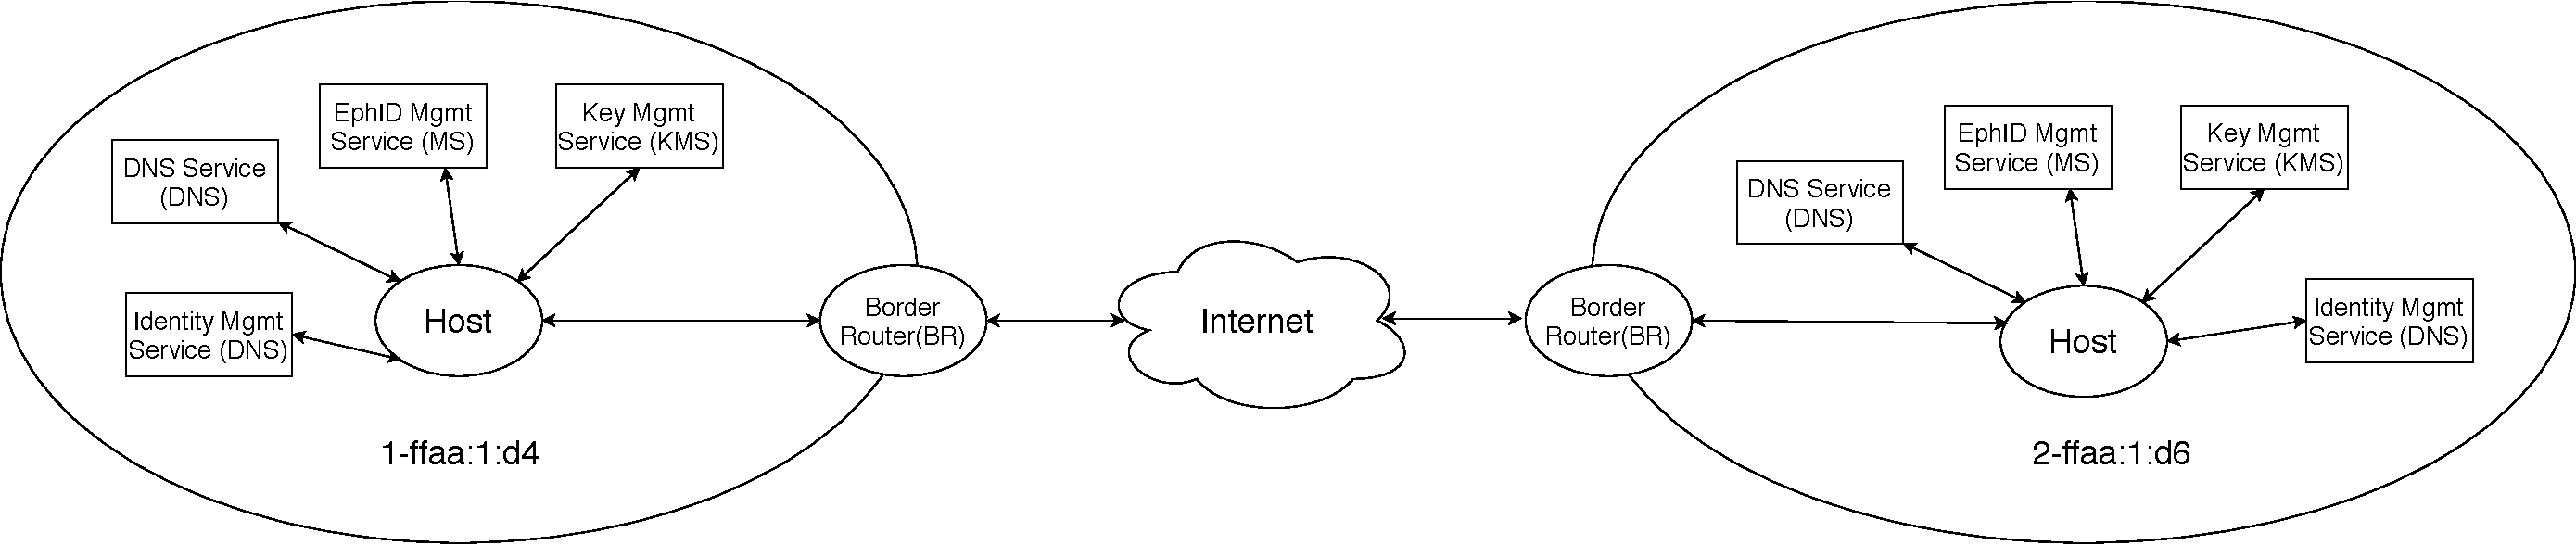
\includegraphics[scale=0.4]{Figures/end_to_end_comm.pdf}}
\decoRule
\caption[APNA End-to-end communication]{An end-to-end communication example}
\label{fig:end_to_end_comm_apna}
\end{figure}

\begin{itemize}
    \item \textbf{EphID Mgmt Service}: issues EphID to the host. (Refer Section \ref{sec:apna_ms})
    \item \textbf{DNS Service}: handle DNS related queries like Domain Registration, Domain Resolution etc. (Refer Section \ref{sec:apna_dns})
    \item \textbf{Identity Mgmt Service}: handles Host Identifier related queries for example converting IPv4/IPv6 address to HID and vice-versa (Refer Section \ref{sec:ims})
    \item \textbf{Key Mgmt Service}: authenticates and bootstraps hosts in the AS. (Refer Section \ref{sec:kms})
    \item \textbf{Border Router}: handles incoming and outgoing packets based on the \texttt{ISD-AS:EphID} tuple.
\end{itemize}

In Figure \ref{fig:end_to_end_comm_apna}, a host in \texttt{ISD-AS(1-ffaa:1:d4)} initiates a communication with host in \texttt{ISD-AS(2-ffaa:1:d6)}. Communication proceeds as described below:

\begin{itemize}
    \item \textbf{Host Bootstrapping:} the host authenticates to the KMS of its AS and registers it's shared secret with the AS and receives the bootstrapping information.
    \item \textbf{EphID Issuance}: the host contacts the EphID Mgmt Service of its AS to obtain an EphID.
    \item \textbf{DNS Operation}: the host either registers its domain name with the DNS service of its AS or the host queries for EphID of the registered domain name.
    \item \textbf{Data communication}: the host proceed with data communication using its \texttt{ISD-AS:EphID} tuple and their peers \texttt{ISD-AS:EphID} tuple which they obtain through DNS Service. If host want to encrypt their communication, they perform a connection establishment prior to the actual communication, to negotiate a shared key that will be used to encrypt their data packets. The shared key is derived from public keys that are associated with the EphIDs.
\end{itemize}

\section{APNA Protocol Details}
The main objective that we had in mind while designing APNA that it should be lightweight and efficient architecture and due to that following design choices were made:

\begin{itemize}
    \item Use of symmetric encryption heavily as compared to asymmetric encryption for example:
    \begin{itemize}
        \item In order to link EphIDs with HIDs symmetric encryption is used; this allows EphID Mgmt Service to efficiently obtain EphID from HID and vice-versa without using a mapping table, which can be large.
        \item Forwarding devices while verifying packet authenticity only perform symmetric cryptography, guaranteeing high forwarding performance.
    \end{itemize}
    \item Proof of sending the packet is embedded inside the packet, avoiding large amounts of stored state as ASes. 
\end{itemize}

\subsection{Assumptions}

\begin{itemize}
    \item We assume that the cryptographic primitive we use are secure. For instance we assume that authenticated encryption used for encrypting data communication is safe against chosen-ciphertext attacks (i.e., CCA-secure). We also require that EphID generation process is also CCA-secure and in future chapters we would describe an efficient CCA-secure encryption scheme to generate EphID.
    \item Every AS has a public key and a corresponding certificate; and there is a public-key infrastructure (e.g., RPKI) from which entity can retrive and verify AS-certificate. Fortunately inside SCION we have Certificate Server (\ref{sec:cert_server}) which contains AS level certificates provides the whole public key infrastructure.
    \item Hosts do not use connection sharing devices (e.g. NAT)
\end{itemize}
\newpage
\bgroup
\def\arraystretch{1.5}%
\begin{center}
\captionof{table}{Notation} \label{tab:notation} 
\begin{tabular}{r  l}
  \hline			
  $k_{A_{i}}$ & Symmetric key of $AS_i$ that is known among the infrastructure (e.g., routers, IMS, KMS)\\
  $k_{H_{i}A_{i}}$ & Symmetric key shared between host $H_i$ and its AS ($AS_i$) \\
  $K_{E_{i}E_{j}}$ & Symmetric key generated for the EphID pair $E_i$ and $E_j$ \\ 
  $HID_i$ & Host identifier (HID) assigned to host $H_i$ \\
  $EphID_h$ & An EphID issued to host $H$ \\
  $C_{EphID_{i}}$ & Certificate for EphID $EphID_i$ \\
  $K^{+}_{E}$, $K^{-}_{E}$ & Public, private key of entity E for both DH Exchange and Digital Signatures.\\
  $MAC_k(M)$ & Message M and MAC of M using symmetric key $k$ \\
  ${M}_{K^{-}}$ & Message M and Signature of M using private-key $K^{-}$ \\
  $E_{k}(M)$ & Symmetric encryption of M with key $k$. \\
  $E^{-1}_{k}(C)$ & Symmetric decryption of C with key $k$ \\
  \hline  
\end{tabular}
\end{center}
\egroup

\subsection{Host Bootstrapping}
A host authenticates to its AS using a well-established authentication protocol. For example, when a user subscribes to an Internet service provider, the provider creates the authentication credentials, and these credentials are preconfigured into an Internet access device (e.g., cable or DSL modem). The device performs the authentication protocol when the user connects it to the network.

The host (or his access device) creates a symmetric key $k_{HA}$ which serves multiple purpose. For example encrypting EphID request and reply message (refer Sec \ref{sec:why_encrypt}) and authenticating every packet that the host sends to the network. During authentication host securely sends $k_{HA}$ to the Key Management Service (KMS) by encrypting it using AS's public key ($K^{+}_{AS}$). 

Once the host is successfully authenticated, KMS of the AS performs the bootstrapping. During this procedure KMS creates a control EphID ($EphID_{h}^{ctrl}$) for the host which is later required for communicating with EphID Mgmt. Service or registering domain name with the DNS service. 

KMS stores the host information ($HID$, $k_{HA}$) and provides API for infrastructure entities to access in the AS e.g., Border Routers, EphID Mgmt. Service, Identity Mgmt. Service etc. The infrastructure will need this information in order to handle packets that are originating from and destined to this host. Specifically, the entities need to learn the HID of the host($HID$) and the shared key ($k_{HA}$) so that they can verify the authenticity of the packets that originate from the host.

Finally the KMS returns the control EphID ($EphID_{h}^{ctrl}$) with its expiration time ($ExpTime$)

\begin{figure}[th!!]
\centering
\noindent
\makebox[\textwidth]{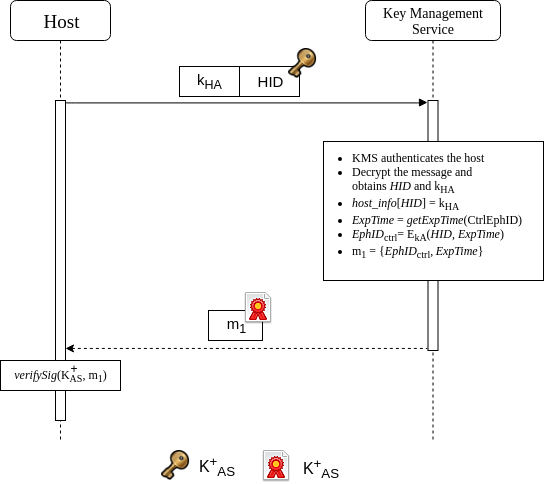
\includegraphics[scale=0.6]{Figures/kms.png}}
\decoRule
\caption[Host Bootstrapping]{Host bootstrapping with Key Management Service}
\label{fig:perf_dns}
\end{figure}

\subsection{Ephemeral ID Issuance}
An EphID is an encrypted token using the AS's secret key ($k_A$). It contains the host's $HID$ and expiration time that indicates the validity period for the EphID. One important point to note is that use of encryption instead of huge mapping tables enables issuing of EphID in a stateless fashion.

Each EphID is associated with a public/private key pair ($K^{+}_{EphID}$, $K^{-}_{EphID}$) which serves three purposes.
\begin{itemize}
    \item Mutual authentication with the peer host
    \item Help in Diffie-Hellman Key Exchange for obtaining the shared key with the peer host for data encryption
    \item Authenticate shutoff requests
\end{itemize}

To keep the data encryption key secret from AS, the host (not the AS) generates the key pair, and the private key is never revealed to the AS. The AS certifies the binding between an EphID and a public/private key pair by issuing a certificate ($C_{EphID}$) that has the same expiration time as the EphID. From the certificate, a peer host learns the public key ($K^{+}_{EphID}$) that is associated to the EphID as well as the EphID expiration time.

\subsection{Data Communication - APNA Session Key Derivation}
In this section, we will discuss about how hosts encrypt their communication and how APNA border routers forward the data packets.

\subsubsection{Data Communication with Network-Layer Encryption}
In order to encrypt the communication between hosts, they need to agree on shared symmetric key which would be used to encrypt the whole communication session. In order to derive this shared symmetric key hosts will perform Diffie-Hellman Key exchange. Note that two hosts can create multiple communication sessions and each session has a different symmetric key to ensure that disclosure of one encryption key does not compromise data privacy of other communication sessions.

Consider two hosts, A and B with EphIDs 
% Chapter apnams

\chapter{APNA Management Service} % Main chapter title

\label{apnams} % For referencing the chapter elsewhere, use \ref{apnams}

\section{What is APNA Management Service}
APNA Management Service is a collection of four different types of services

\begin{itemize}
    \item Ephemeral ID Management Service
    \item Domain Name Service (DNS)
    \item Key Management Service (KMS)
    \item Identity Management Service (IMS)
\end{itemize}

\section{Ephemeral IDs Management} \label{sec:apna_ms}
Ephemeral IDs (EphIDs) are very important component needed for establishing anonymous and accountable communication between host. Thus a major responsibility of the management service is to issue this EphID very efficiently as it would be required by every host trying to establish a new communication. This should also meet the security guarantees that is required from EphIDs. In order to efficiently compute EphID instead of keeping huge mapping inside the table symmetric cryptography is used to implement it in a stateless fashion.

\subsection{Ephemeral ID (EphID) Structure}
We engineered the length of EphID to optimize processing for the AES block cipher as its the only cipher with widespread hardware support, which enables high performance. In order to generate EphIDs we use a CCA-secure encryption scheme. To this end, we use a generic composition called Encrypt-then-MAC that combines a symmetric encryption with a message authentication code (MAC).
Ephemeral IDs are composed of three things:
\begin{itemize}
    \item Initialization vector (IV)
    \item Encrypted Host Identifier (EHID)
    \item Message Authentication Code (MAC)
\end{itemize}

\begin{figure}[th]
\centering
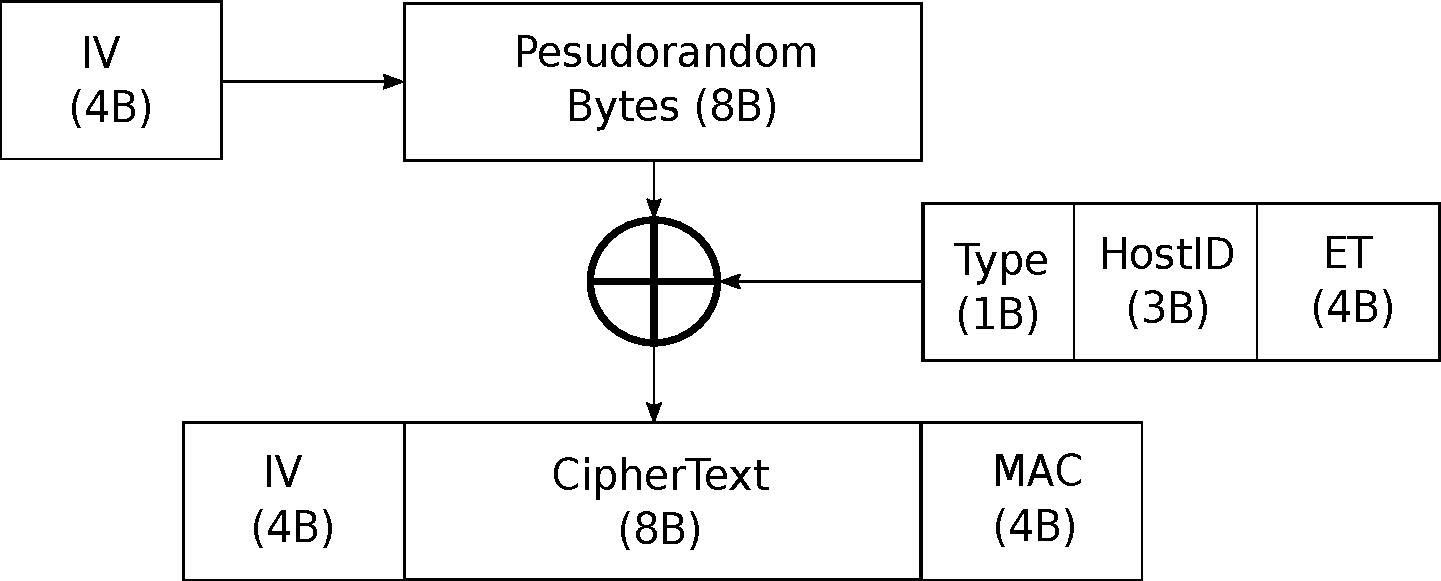
\includegraphics[scale=0.5]{Figures/ephid_construction.pdf}
\decoRule
\caption[EphID Construction]{EphID Construction, where ET is Expiration Time}
\label{fig:ephid_con}
\end{figure}

\subsubsection{Initialization Vector (IV)}
Secure operations of this mode in AES requires a unique IV for every encryption operation (i.e. for every EphID)

\subsubsection{Host Identifiers (HID)}
\begin{center}
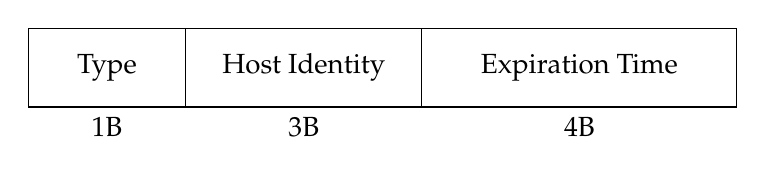
\begin{tikzpicture}
    \draw (0,0) rectangle (2,1) node[pos=.5] {Type}; %node[anchor=north, pos=.5]{0};
    \draw (2,0) rectangle (5,1) node[pos=.5] {Host Identity};
    \draw (5,0) rectangle (9,1) node[pos=.5] {Expiration Time};
    \draw (1 cm,0pt) -- (1 cm,0pt) node[anchor=north] {1B};
    \draw (3.5 cm,0pt) -- (3.5 cm,0pt) node[anchor=north] {3B};
    \draw (7 cm,0pt) -- (7 cm,0pt) node[anchor=north] {4B};
\end{tikzpicture}
\end{center}
Host Identifiers has three main components:
\begin{itemize}
    \item \textbf{Type:} There are two types Control EphID and Session EphID. Control EphID is mainly used to communicate with AS related services. On the other hand Session EphID is used for negotiating a session between client and server. It is also used during the whole communication process.
    \item \textbf{Host Identity:} Host is the 3 byte unique representation for all the host within the AS. It's sufficient enough to uniquely represent all host even in the large ASes.
    \item \textbf{Expiration Time:} This represents the validity of an EphID which is expressed in Unix seconds. Control EphID usually have a longer expiration time than Session EphID. For example in our implementation Control EphID has an expiration time of 1hour and Session EphID has an expiration time of 5mins.
\end{itemize}

\subsubsection{Message Authentication Code (MAC)}
IV and EHID are signed with the HMAC so that it could verify MAC before decryption of EphID to find HID to forward the packet.

\subsection{EphID Issuance} \label{sec:why_encrypt}
To obtain an EphID, the host generate public/private key pair ($K^{+}_{EphID}$, $K^{-}_{EphID}$) and send an EphID creation request to MS as shown in Figure \ref{fig:ephid_gen}. Specifically, the host first generates the key pairs for the EphID and include $K^{+}_{EphID}$ (\texttt{0xcafe}) along with type (\texttt{CtrlEphID}) and address of the domain name (\texttt{www.abc.com}) in the request message. All the communication with APNA Management Service is encrypted with using the shared key with the AS ($k_{HA}$). The public key in the message is encrypted to hide it from other entities in the AS that are not part of the AS infrastructure.

If an adversary trying to compromise sender-X unlinkability sees the content of EphID request packets, he/she can idenitfy a common sender at the level of $EphID_{Ctrl}$. Specifically the adversary first learns the ($EphID_{Ctrl}$, $K^{+}_{EphID}$) pair from the EphID request packets; then, the addversary sees the $K^{+}_{EphID}$ from the connection establishment packets, allowing the adversary to identify the common sender of multiple connections. Note that the actual host identity is still not compromised since only the host's AS can extract the host identity from $EphID_{Ctrl}$. In APNA, encrypting the EphID request message prevents such attacks.

Upon receiving the request, the EphID Mgmt Service validates the authenticity of the request; decrypts the source EphID ($EphID_{Ctrl}$) and performs the following check
\begin{itemize}
    \item $EphID_{Ctrl}$ has not expired
    \item the client's identifier ($HID$) is valid i.e, has not been revoked
    \item the request message is valid and can be decrypted successfully.
\end{itemize}
If anyone of them fails client gets a reply back with specific \textit{ErrorCode}. If its succesful then EphID Mgmt. Service generates an EphID and a certificate ($C_{EphID}$) corresponding to it and send it back as a response. The certificate is encrypted for the same reason as encrypting the EphID request packets.

\begin{figure}[th!!]
\centering
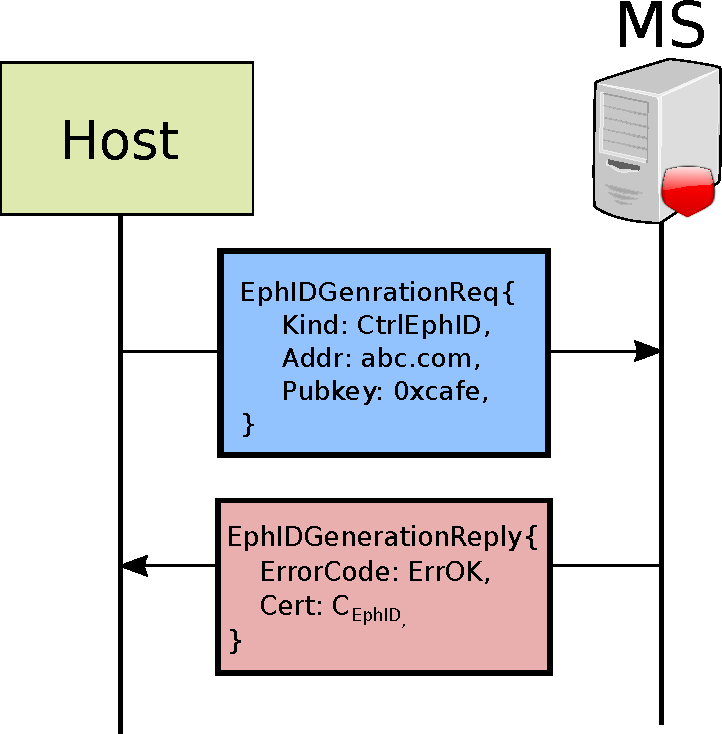
\includegraphics[scale=0.6]{Figures/ephid_gen.pdf}
\decoRule
\caption[EphID Generation Request]{Control EphID generation request by abc.com}
\label{fig:ephid_gen}
\end{figure}

\begin{figure}
    \centering
        \begin{bytefield}{32}
            \bitbox{32}{Ephemeral ID := $I_i$ (16 bytes)}\\
            \wordbox{1}{Pubkey (32 bytes)}\\
            \wordbox{1}{Expiration Time (4 bytes)}\\
            \bitbox{32}{Signature (32 bytes)}
        \end{bytefield}
        \decoRule
        \caption{Certificate byte level representation \tiny{\textsc{not to scale}}.}
        \label{fig:ephid_cert}
\end{figure}

\subsection{Certificate Structure}
In order to get more exact details about internals of the certificate associated with an EphID look at Figure \ref{fig:ephid_cert}. Signature is calculated using Elliptic Curve Cryptography (Ed25519) and thus the host can verify the authenticity of the issued certificate using the AS's public key which issued the certificate.

\section{Domain Name Service (DNS)} \label{sec:apna_dns}
\subsection{Why can't we use current DNS system?}
Since in APNA we have replaced IP addresses with Ephemeral Addresses which makes the current DNS system completely obsolete. Currently, DNS only understands how to resolve URL to IP addresses but in order to communicate with other APNA host we would need Ephemeral Address. In order to solve this problem current DNS could be modified be instead of returning A/AAAA records, it could return the certificate associated with the Ephemeral ID. This certificate contains all the details needed to establish the communication between communicating parties.

\subsection{Problems with publishing EphID to DNS}
Publishing EphIDs to the DNS raises a problem: a shutoff request against a published EphID would terminate any ongoing communication sessions that use this EphID. A naive solution is to update with a new EphID whenever published EphID becomes invalid. However an attacker can DDoS the DNS infrastructure by continuously sending shutoff request against a domain.

Our solution is to use Control EphIDs that are only used for to receive packets and are never used as the source EphIDs. Since they are never used as the source identifier, they cannot become the target of shutoff requests. To avoid using receive-only EphIDs as the source identifier, the communication establishment to a server needs to be changed (i.e., server does not respond to the client using the receive-only EphID).

\subsection{Details}
It's a simple prototype implementation for DNS which works on basic register and request based protocol. For instance a server could register its certificate associated with receive only EphID with DNS when it starts. Whenever a client would need to fetch the server identity it could request from DNS Service. Internally its implemented using Golang map data structure whose complexity for insertion and lookup is $\mathcal{O}(1)$ which makes it a perfect candidate for the prototype. This makes DNS operation very fast and efficient.

\subsection{DNS Operations}
\subsubsection{DNS Registration}
Figure \ref{fig:dns_register} represents a scenario in which a server registers \texttt{abc.com} receive only EphID's certificate ($C_{EphID}$) with the DNS service and if its successful it sends \texttt{ErrOk} back to the server.

\subsubsection{DNS Resolution}
Figure \ref{fig:dns_request} represents a scenario in which a client request for \texttt{abc.com} receive only EphID's certificate ($C_{EphID}$) with the DNS service and if the \texttt{abc.com} is registered with the DNS service it will reply with its $C_{EphID}$

\begin{figure}[th!]
\centering
\begin{subfigure}{.5\textwidth}
  \centering
  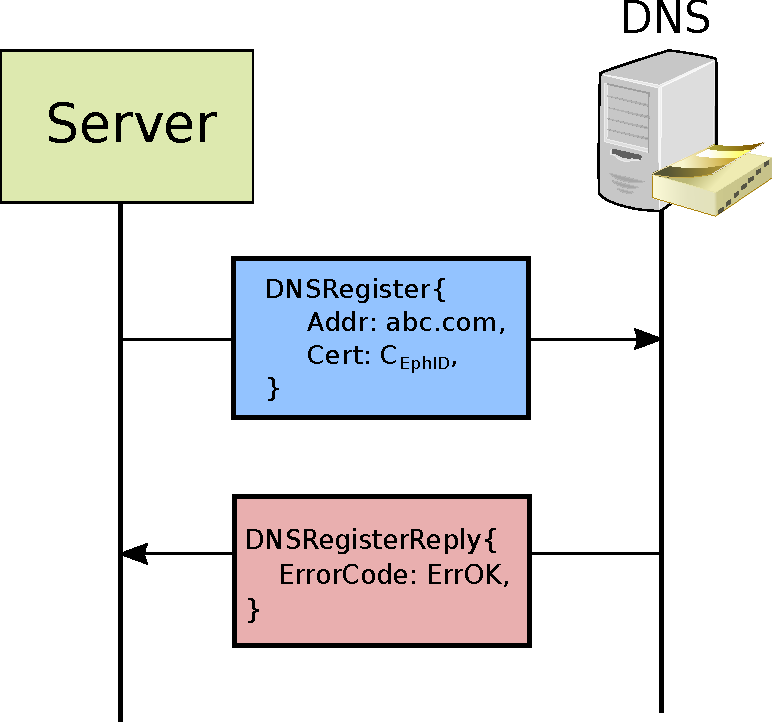
\includegraphics[width=0.95\linewidth]{Figures/dns_register.pdf}
  \caption[DNS Register Domain]{abc.com registers $C_{EphID}$ with DNS}
  \label{fig:dns_register}
\end{subfigure}%
\begin{subfigure}{.5\textwidth}
  \centering
  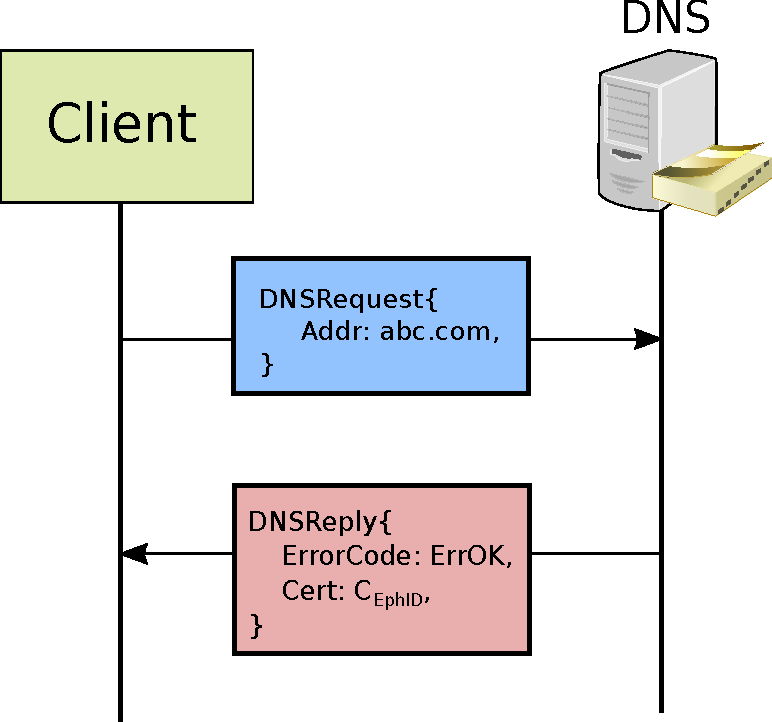
\includegraphics[width=0.95\linewidth]{Figures/dns_request.pdf}
  \caption[DNS Request for a Domain]{Client query abc.com's $C_{EphID}$ from DNS}
  \label{fig:dns_request}
\end{subfigure}
\caption{DNS Register and Request Methods}
\label{fig:dns}
\end{figure}

\section{Message Authentication Key Management} \label{sec:kms}
In APNA every packet contains MAC signed by the symmetric key of the host which is sending the packet. The symmetric key which is used to sign the packet is registered with the Management Service. So the forwarding service could ask the management service for this key and verify the authenticity of the packet before forwarding the packet to the rest of network.

\begin{figure}[th!]
\centering
\begin{subfigure}{.5\textwidth}
  \centering
  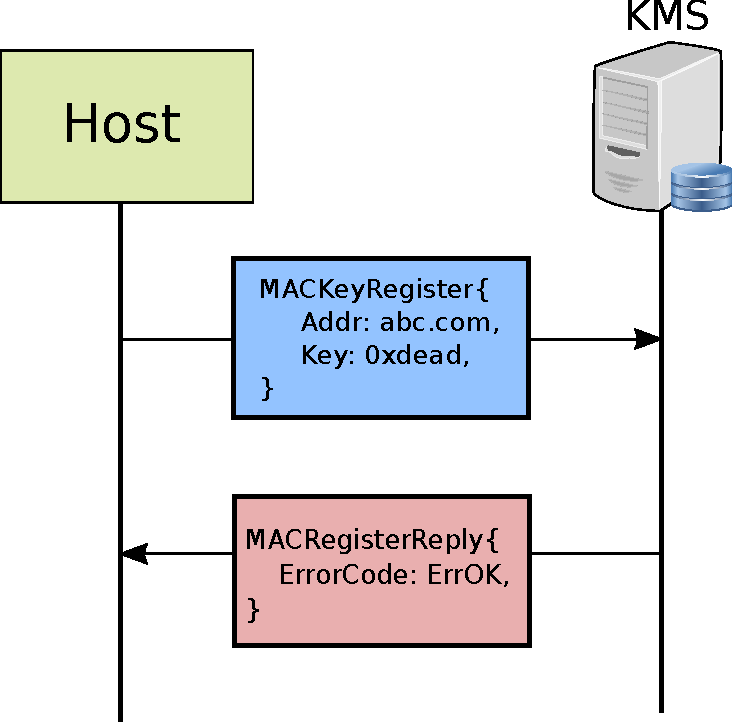
\includegraphics[width=0.95\linewidth]{Figures/kms.pdf}
  \caption[MAC Key Register]{Register Key}
  \label{fig:kms_register}
\end{subfigure}%
\begin{subfigure}{.5\textwidth}
  \centering
  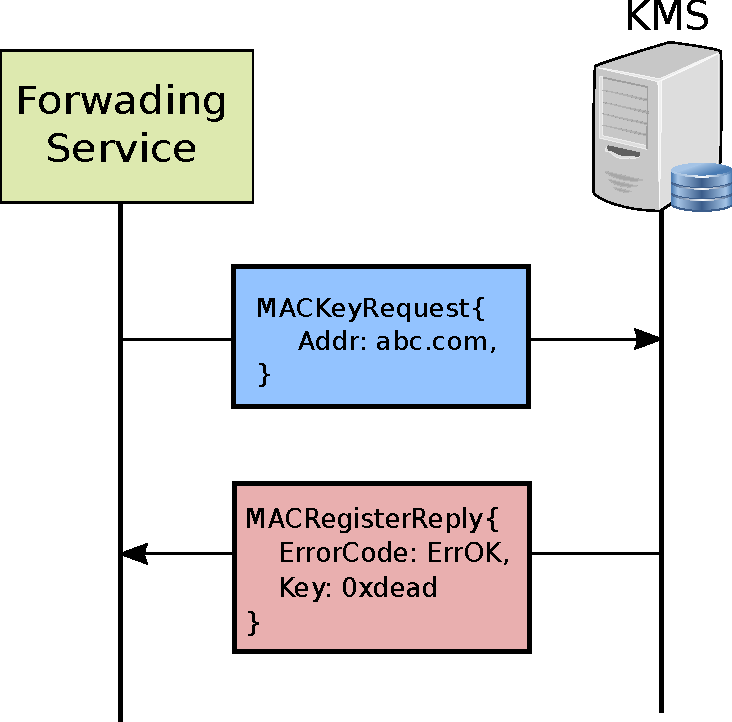
\includegraphics[width=0.95\linewidth]{Figures/kms_request.pdf}
  \caption[MAC Key Request]{Request Key}
  \label{fig:kms_request}
\end{subfigure}
\caption{Key Management Service}
\label{fig:kms}
\end{figure}

\section{Mapping IPv4/IPv6 addresses to Host Identity} \label{sec:ims}
Current internet only understands IPv4/IPv6 addresses to route any packet on the internet. In order to route APNA packets we need to build overlay network over the current internet. On other hand we also need 3 bytes unique representation for each host within the AS. So we have used Siphash [??] to create unique 3 bytes representation from IP address.

\begin{figure}[th!]
\centering
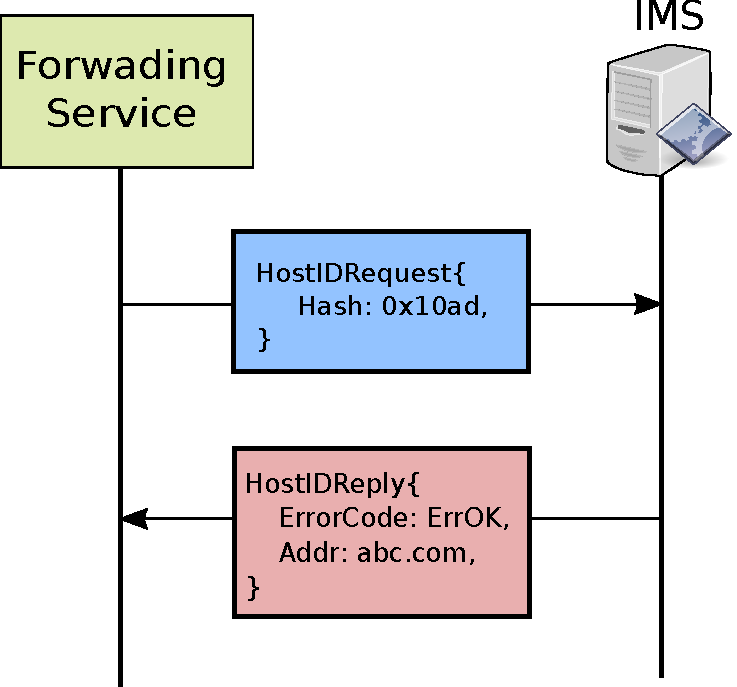
\includegraphics[scale=0.6]{Figures/siphash.pdf}
\decoRule
\caption[Host Identity Service]{Forwarding Service request IP address for a host identity from Identity Management Service (IMS)}
\label{fig:ims_request}
\end{figure}

\section{Implementation}
All the API access to APNA Management Service are modeled using Cap’n Proto specification.
% Chapter APNA Overlay

\chapter{APNA over SCION} % Main chapter title

\label{apna_overlay}
In order to integrate APNA inside there are few key challenges:
\begin{itemize}
    \item Replacing IP addresses with Ephemeral Identifiers for the communication purpose. 
    \item Modifying the packet forwarding service (i.e., border routers) to incorporate the packet authenticity checks and packet forwarding based on the Ephemeral Identifiers.
\end{itemize}

There are multiple ways to overcome those challenges and we discuss three different ways to integrate APNA inside SCION and they are as follows:
\begin{itemize}
    \item APNA over SCION (Chapter \ref{apna_overlay})
    \item APNA address family (Chapter \ref{address_family})
    \item APNA as SCION Service (Chapter \ref{apna_service})
\end{itemize}

In this chapter we will discuss the first approach to implement APNA as a overlay on the current SCION infrastructure and the rest of the approaches are discussed in further chapters. We will start with the explaining the core idea behind this approach (Section \ref{overlay:main_idea}), proceeding with technical difficulties and modification required in the current infrastructure (Section \ref{overlay:modifications}). After that we will talk about example scenario in which two hosts will establish a communication session interacting with services from APNA Management Service (Section \ref{overlay:comm}) and in the end we will discuss some shorting or drawbacks related to this approach (Section \ref{overlay:drawback}).

\section{Main Idea} \label{overlay:main_idea}

The main idea behind this approach is to encapsulate APNA packet as a payload to the SCION packet. This idea is very similar to how TLS is implemented over TCP or how QUIC is implemented over UDP.  QUIC uses UDP as substrate so as to not require changes to legacy client operating systems and middleboxes to be deployable.

\subsection{Why APNA is built on top of SCION?}
Following a similar reasoning to QUIC/TLS \cite{quic} \cite{tls}, APNA is also built on top of SCION. The reason behind that it requires least amount of modification in the current SCION infrastructure which makes its deployment very easy on SCIONLab or other SCION deployments. Since it is not dependent on other SCION infrastructure, this loose coupling with other components helps a lot in the development of APNA protocol.

\subsection{What happens to SCION Intra-Domain Header?} \label{overlay:miss_l4}
For SCION all the information related to intra-domain routing is available inside L4 header. And primarily intra-domain routing is based on IP address for SCION. But we don't want IP address in the SCION packet as that will result in the violation of sender-X unlinkability property of APNA protocol. So in order to overcome this problem instead of using real IP addresses in the L4 header for source and destination address we replace it with some identification tag for APNA Packet. For the sake of implementation we reserved the "apna" ASCII representation i.e., \texttt{97.112.110.97} (IPv4 address) or \texttt{0:0:0:0:0:FFFF:6170:6E61} (IPv6 address) to identify whether its APNA packet or not.

\section{Modification in the current infrastructure} \label{overlay:modifications}
There are various reasons due to which we require some modifications in the SCION infrastructure and those reasons are as follows:
\begin{itemize}
    \item Source border routers need to authenticate the packet before forwarding the packet, as its one of the requirements of the APNA protocol. Thus source border router needs to performs extra packet processing as compared to rest of the border routers in the network.
    \item Since there is no destination address in the L4 header (Section \ref{overlay:miss_l4}) hence the destination border router cannot forward the packet to the right dispatcher which would eventually forward it to the correct host.
    \item Modification are required in the current SCION packet structure to accommodate APNA header inside its payload.
    \item User-space library SNET which is used to establish communication inside SCION also needs to be modified as there are changes in the packet parsing with new APNA header.
\end{itemize}

\subsection{Border Router (BR)}

\paragraph{Source Border Router Modifications} \label{overlay:br_src}
Source BR needs to verify packet authenticity before the packet can the leave the host AS. In order to verify packet authenticity BR would needs to find the sender of the packet which can obtained by parsing payload into an APNA packet. After parsing the packet it could inspect source EphID and decrypt it to obtain host's $HID$. But in order to decrypt it would require $k_{AS_{i}}$ with which it was encrypted initially. This can be solved by passing an extra configuration file while starting the border router which will contain the $k_{AS_{i}}$.

Once it has successfully decrypted the HID it could contact the Key Mgmt. Service (Section \ref{sec:kms}) in order to obtain the shared key ($k_{HA}$) with which the packet is signed. That raises another problem how to contact the KMS and that could solved by using same the configuration file by including the IP address and Port Number at which KMS is listening. All the communication between BR and KMS needs to be encrypted and symmetric key associated with that encryption is also present inside the same configuration file. More details about this configuration file is present in Section [??]

Contacting KMS every time a packet comes in could be expensive. So it implements a small cache of replies which it received from the KMS for fast packet processing. Currently it's a very simple cache based on First in First Out (FIFO) replacement policy, but it would be interesting to investigate other caching policies such as Least Recently Used (LRU) etc.

After successfully authenticating the packet source BR could forward using path information available inside the SCION packet.

\paragraph{Destination Border Router Modifications} \label{overlay:br_dst}
After the modifications suggested in the aforementioned section packet will the reach the destination BR. If it was a normal packet then BR would have looked at the destination IP address in the L4 header and forwarded it to that dispatcher with that IP address and  \texttt{EndhostPort} (30041) with its existing UDP overlay. But the destination IP address in the L4 header is replaced with random IP address so that operation is no longer valid.

In order to obtain correct IP address of the dispatcher it needs to needs to parse the packet and obtain destination EphID. Using that EphID, BR could decrypt it to obtain destination host's $HID$ and after that it could contact the IMS (Section \ref{sec:ims}) to obtain the IP address. But the dispatcher only understands IP address, so border router performs the translation from HID to IP address and updates the SCION packet L4 destination address.

It is kind of obvious that more APNA packets are coming with same HID in the future thus it can perform some caching on the results from IMS for faster packet processing such as source BR.

\subsection{SCION-APNA Packet Structure}
\begin{figure}[th!!]
\centering
\noindent
\makebox[\textwidth]{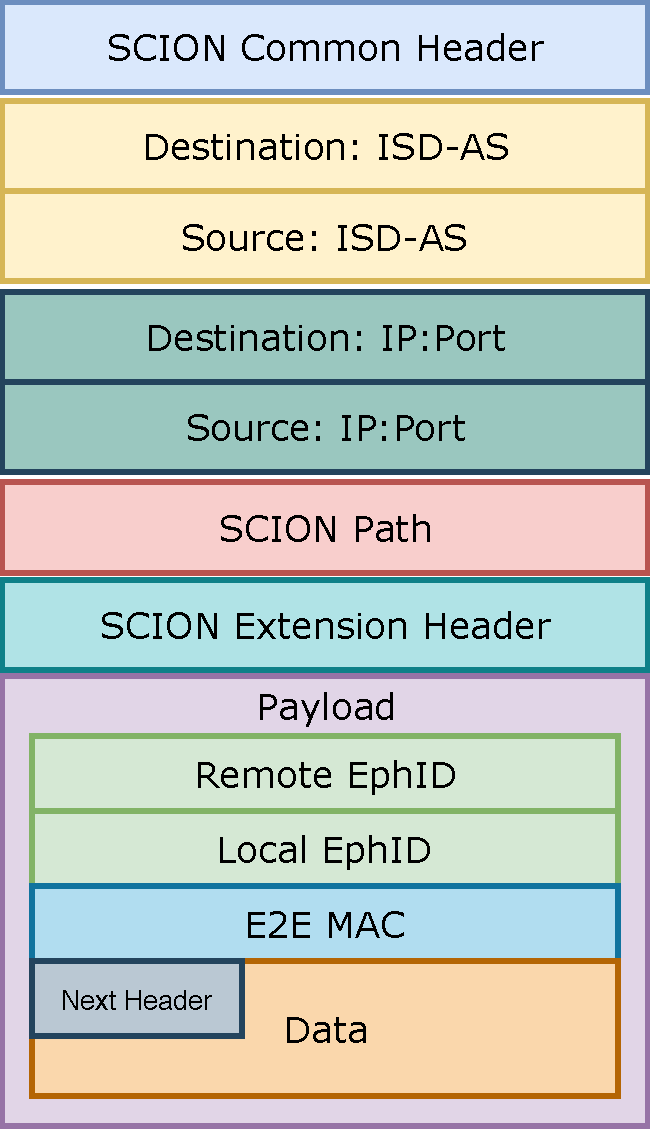
\includegraphics[scale=0.6]{Figures/apna_inside_scion.pdf}}
\decoRule
\caption[APNA packet structure inside SCION]{APNA Packet inside SCION Payload}
\label{fig:apna_scion_pkt}
\end{figure}

Figure \ref{fig:apna_scion_pkt} represents a modified SCION packet encapsulating APNA packet inside it as a payload. IP addresses shown in the above packet are filled with random address while constructing the packet.

\subsection{SNET} \label{overlay:snet}
Since we no longer wants to use IP address for our communication the main networking library needs to be modified to accommodate that request. In order to accomplish this \texttt{snet.ListenSCION()} and \texttt{snet.DialSCION()} needs a accept a new network string parameter "\texttt{apna}". Before this it only supported "\texttt{udp4}". Accordingly the \texttt{read} and \texttt{write} methods provided by interface \texttt{snet.Conn} also needs to be modified as they deal with creating and parsing the SCION packet. Currently IP address for source and destination are set to actual ones corresponding to the host. But since we want to hide those IP addresses we can redact it with some random address as its not needed for intra-domain forwarding. For inter-domain forwarding last hop border router fills in with the correct IP address.

\paragraph{APNA Session Management}
APNA session consists of following components:
\begin{itemize}
    \item \texttt{SessionPrivateKey}:  This private key corresponds two second EphID which contributes to the SessionSecret.
    \item \texttt{SessionSharedSecret}: This shared secret key derived from the pair of second EphID public/private key pairs.
    \item \texttt{PreSessionSharedSecret}: This shared secret key derived from the pair of first EphID public/private key pairs.
    \item \texttt{LocalEphID}: is the host's session EphID
    \item \texttt{RemoteEphID}: is the session EphID of the remote host.
\end{itemize}

\paragraph{APNA Key Exchange inside SNET}
Since the underlying network is still UDP based, so SNET needs to implement the handshake on top this UDP based overlay network. The goal of this handshake is to initialize the aforementioned session structure. In the first part of the handshake \texttt{PreSessionSharedSecret} and  \texttt{SessionPrivateKey} gets populated and in the second part of the handshake rest of the parameters gets initialized.

\section{Data Communication} \label{overlay:comm}
This section describes all the important steps involved in establishing a communication between a client and a server using APNA.
\subsection{SCION Initialization Phase}
This phase is common to all the host which wants to use SCION infrastructure for communicating with the other host of the SCION network. First of all a host needs to initialize the networking context using \texttt{SNET} and register its IP address with dispatcher. In order to initialize three things are required: 1) SCIOND socket path 2) dispatcher socket path and 3) ISD-AS address. An example is shown in \ref{code:scion_init}.

\begin{code}
\captionof{listing}{SCION networking context initialization}
\inputminted[frame=lines, framesep=2mm, baselinestretch=1.2, fontsize=\footnotesize, linenos]{go}{code_snippets/scion_init.go} \label{code:scion_init}
\end{code}

Once a host is successfully registered with dispatcher it can register with the Key Management Service to issue an Control EphID to the host and perform host bootstrapping. After getting Control EphID it can do different stuff depending upon its requirements.

\subsection{Starting APNA Server}
Once the server has obtained a control EphID from the KMS it can contact the EphID Mgmt. Service to issue a receive only control EphID and use that certificate to register with the DNS service. After that it can start a new APNA server listening on a particular address using the APIs provided by \texttt{SNET}.

\subsection{Starting APNA Client}
Once the client has obtained a control EphID from the KMS it can contact the EphID Mgmt. Service to issue two different session EphID which then can be used for APNA Handshake with the server. Then the client can use the simple \texttt{SNET} API called \texttt{snet.DialSCION("apna4", dstAddr, srcAddr)} which would return a \texttt{Conn} interface that could be used to perform APNA handshake and send data further along.

\subsection{Packet Forwarding}
A border router in the source AS ensures that only packets from authenticated hosts and authorized EphIDs leave the AS; and a border router in the destination AS forwards the packets to correct dispatcher based on the destination EphID. Transit ASes do not perform additional operations and simply forward the packets to the next AS mentioned in the SCION header path information. In order to achieve high performance data forwarding, only symmetric cryptographic operations are used.

Communication end-points are specified as ISD-AS:EphID tuples. For inter-domain forwarding, border routers use only ISD-AS to forward packets. Specifically, for external packets entering the AS, a border router checks whether the packet has arrived at the destination AS (Figure \ref{fig:overlay_dst}). If not, the packet is forwarded to the next AS mentioned in the Path Information in the SCION packet (Line 9). At the destination AS, the border router performs the following conditions: 1) the destination EphID ($EphID_{d}$) is valid, i.e., has not expired (Line 4).

If all the conditions are satisfied, then the border router tries to resolve IP address from $HID_{d}$ with the help of APNA Management Service. First border check its own cache of IP address from HID, if the HID is not present in its cache it would sent a host resolution query to the APNA management service. If the APNA Management Service replies with $ErrHostNotPresent$ it drops the packet and abort. If it replies with $ErrorOK$, then border router forwards the packet to the dispatcher by setting the destination IP address with the reply sent from Management Service. Then the dispatcher forwards the packet according to the host mapping it has depending upon the host which registered with it in the first step.

For outgoing packets, a border router forwards the packet to a neighboring AS only if all the following conditions are satisfied: 1) the source EphID ($EphID_{s}$) is valid i.e., has not expired (Line 3 in the \ref{fig:overlay_src}) 2) the MAC in the packet is correct (Line 6).

To verify the MAC in the packet, a border router retrieves the shared key ($k_{HA}$) between the source host and the AS by searching the host information database ($host\_info$). Entries in this database are populated with the help of APNA Management Service using its Key Management Service (\ref{sec:kms})

\begin{figure}[th!!]
\centering
\hspace*{2cm}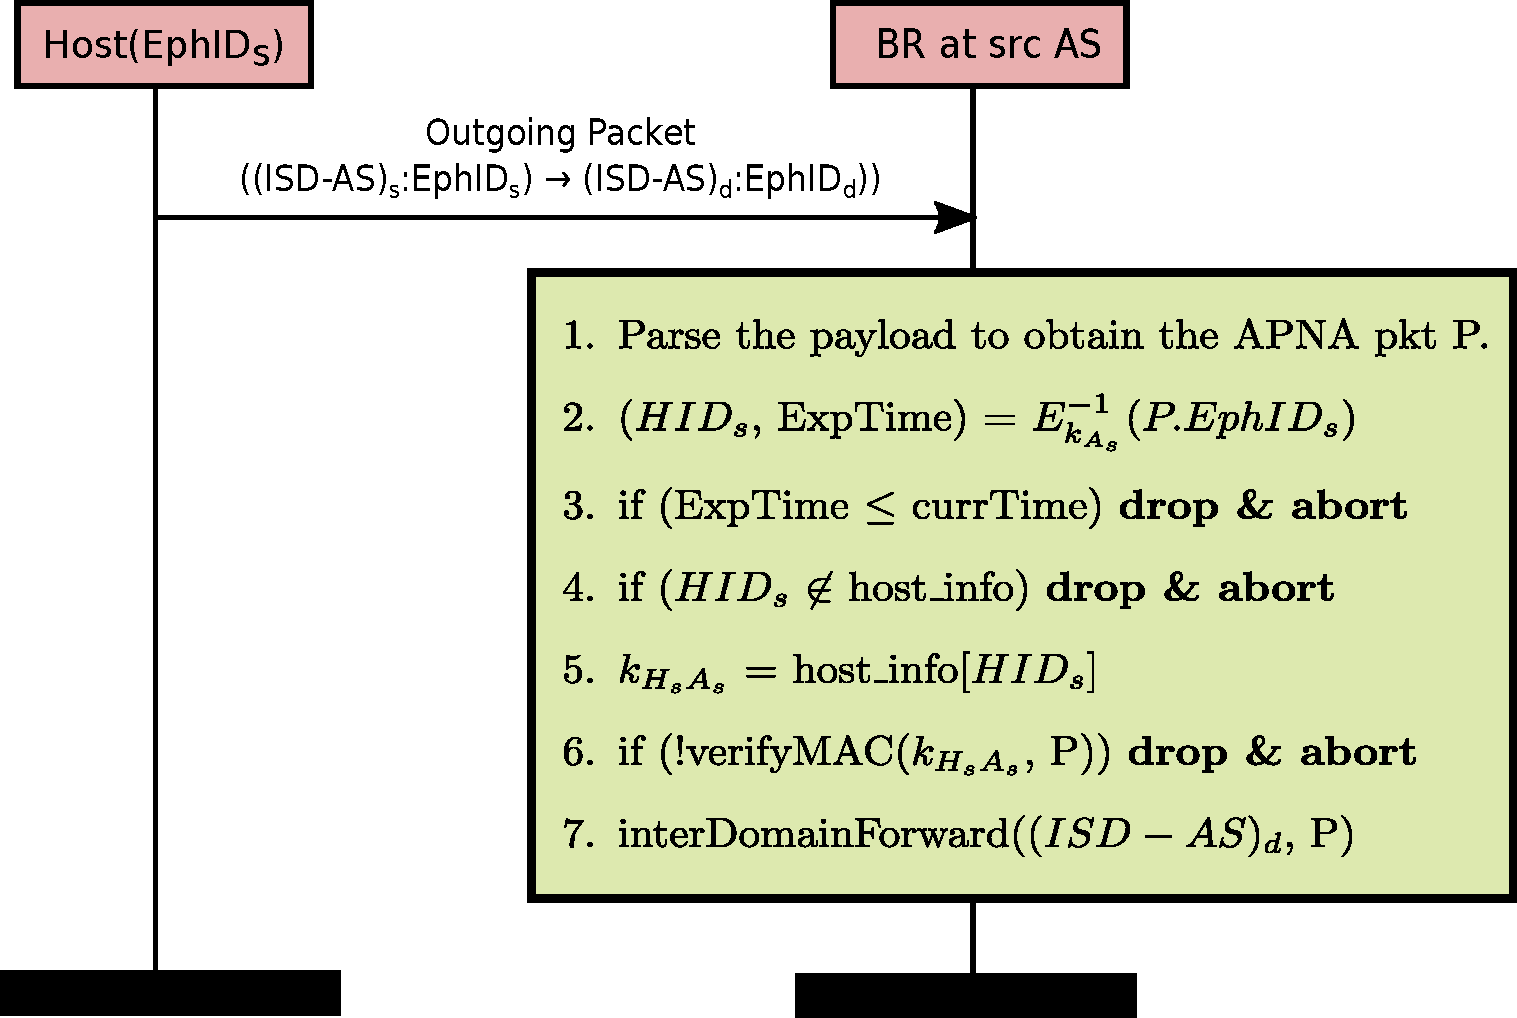
\includegraphics[scale=0.5]{Figures/overlay_src.pdf}
\decoRule
\caption[APNA Overlay Outgoing Packet]{Outgoing Packet}
\label{fig:overlay_src}
\end{figure}

\begin{figure}[th!!]
\centering
\hspace*{2cm}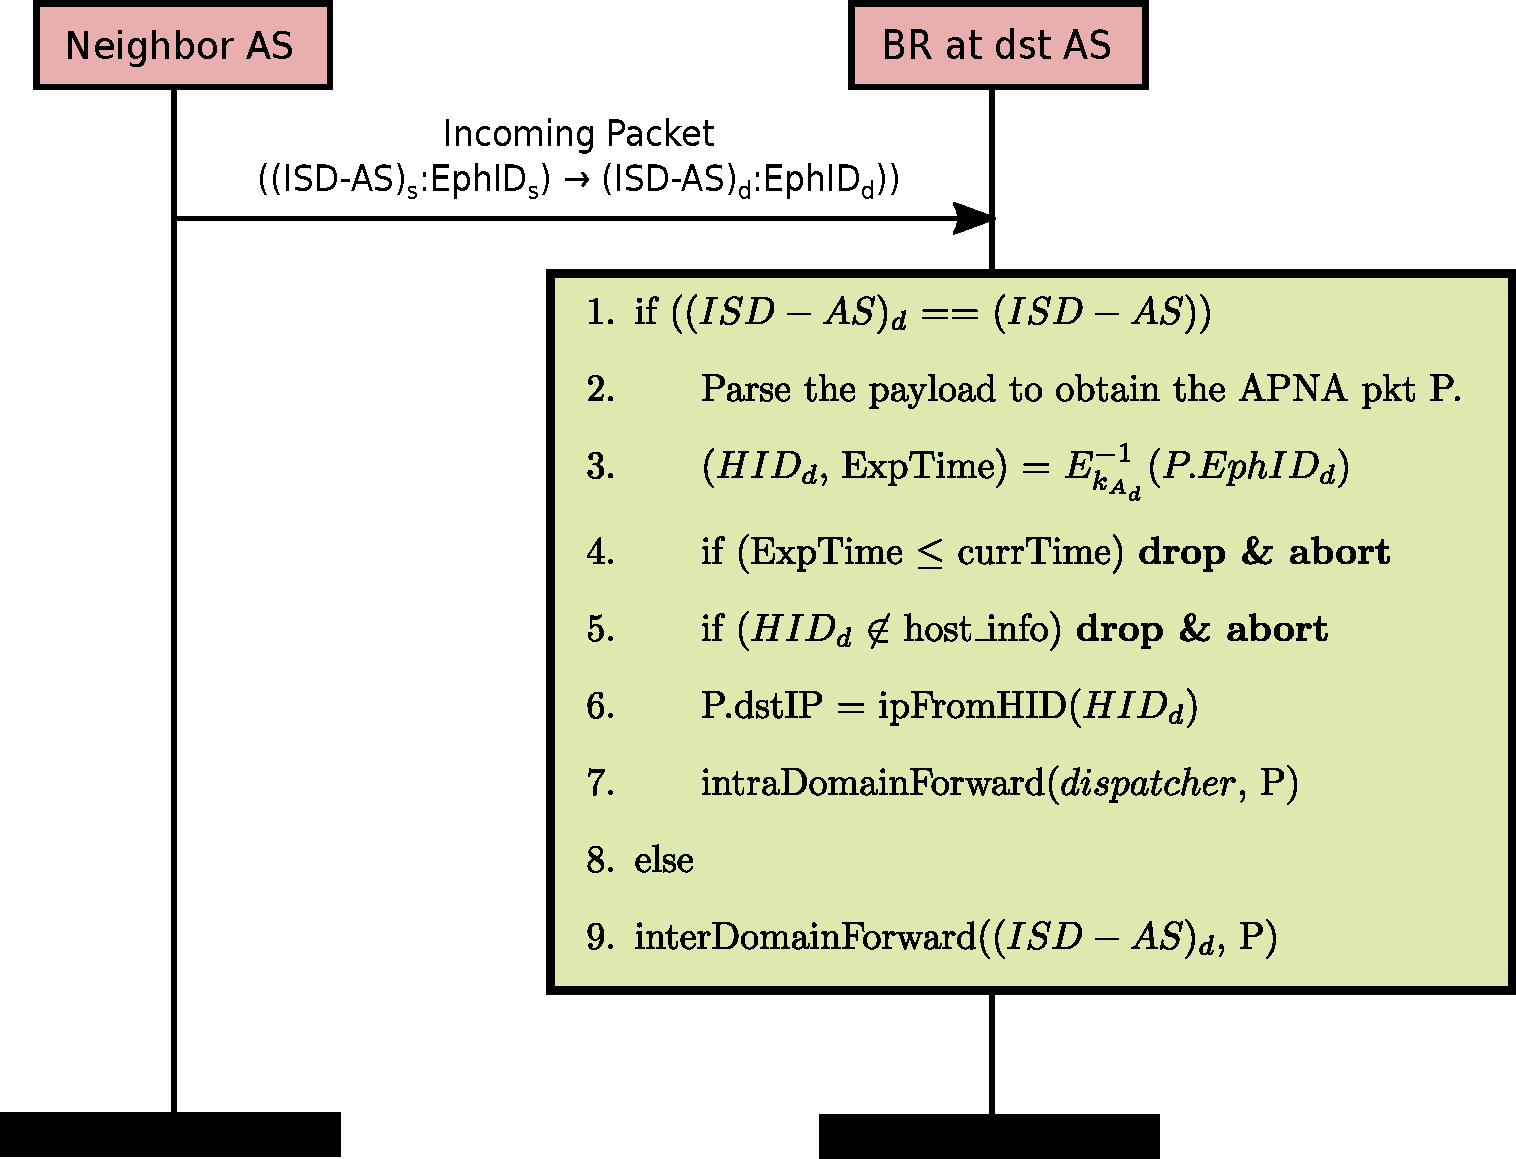
\includegraphics[scale=0.5]{Figures/overlay_dst.pdf}
\decoRule
\caption[APNA Overlay Incoming Packet]{Incoming Packet}
\label{fig:overlay_dst}
\end{figure}

\subsection{APNA Handshake}
In order to derive shared session key using Diffie-Hellman key exchange which would be used to encrypt the traffic between client and server. They need to perform the handshake described in Section \ref{sec:apna_proto}. 

\section{Drawbacks} \label{overlay:drawback}
In the hindsight this approach feels like kind of hack and not very well integrated inside the SCION infrastructure. In a way we are kind of abusing the packet header fields by randomly filling some random marker inside L4 header which otherwise can be used judiciously for user data. This reduces the overall MTU of the SCION packet. The question is can we something better and the answer is yes. But extending the address family which SCION supports and making a new address family for APNA which can then store EphID. More details about this approach will be discussed in the next chapter.
% Chapter AddressFamily

\chapter{AF\_APNA} % Main chapter title

\label{address_family}

% Chapter ApnaService

\chapter{APNA as SCION Service} % Main chapter title

\label{apna_service}

\section{APNA Service}
APNA Service (AP\_SVC) is radically different from the past two approaches described in previous chapters (Chap. \ref{apna_overlay}, \ref{address_family}). The main idea behind this approach is to create a new SCION service (like Path Service, Certificate Service) which would be responsible for forwarding APNA packets. The main advantage of this approach instead of modifying the border router and dispatcher to handle APNA packets this new service will take care of APNA packets instead. That makes this approach easily deployable on the current SCIONLab infrastructure without a lot of changes in the existing deployment.

APNA service is like a data plane service which is responsible for providing anonymous communication service for SCION. Any packet send to APNA service will get anonymously delivered to the destination. Source APNA service uses the anycast address to deliver the packet to destination APNA service which then forwards it to the appropriate host. Since we are using the anycast address for communication attacker cannot hamper the anonymity guarantees provided by APNA framework. 

\subsection{Communication Overview}
\begin{figure}[th!!]
\centering
\hspace*{-2cm}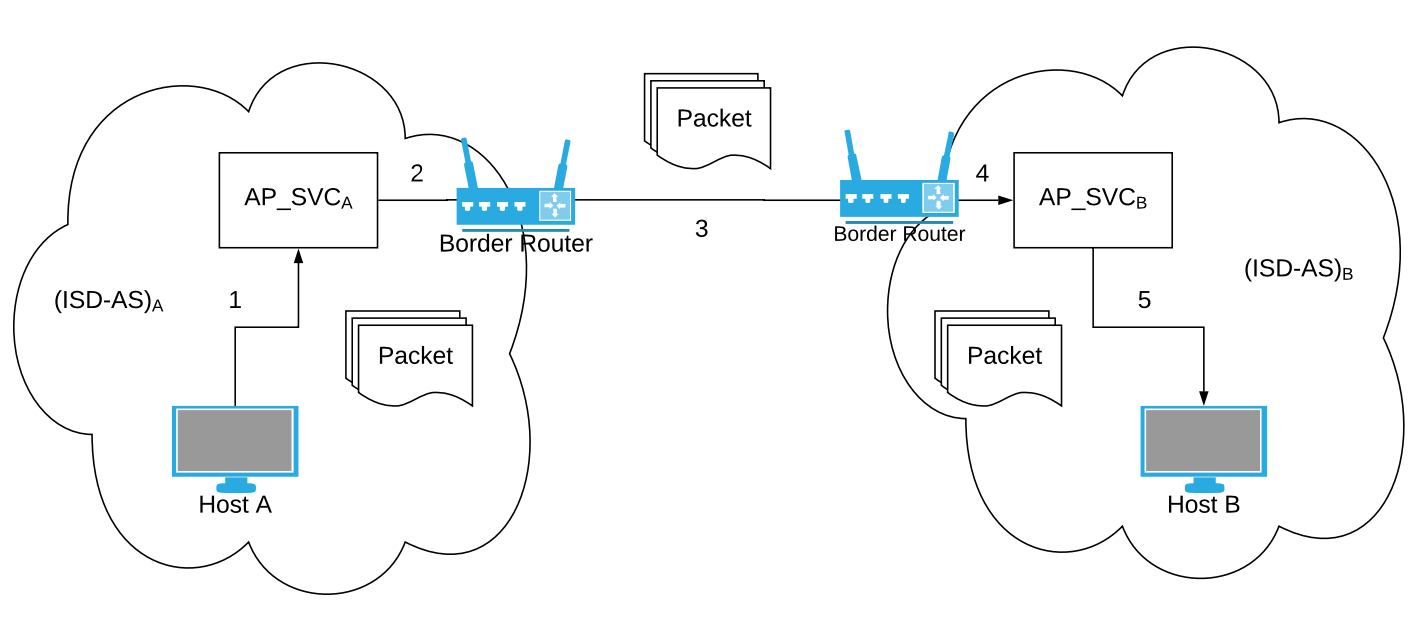
\includegraphics[scale=0.3]{Figures/svc_arch.png}
\decoRule
\caption[Communication overview for APNA Service]{Communication overview for APNA Service architecture}
\label{fig:srv_comm}
\end{figure}
In order to understand how does two parties communication using this new APNA Service. Let's take a simple scenario as presented in Fig.\ref{fig:srv_comm}. In this case Host A which is located in $(ISD-AS)_{A}$ wants to send a packet to Host B located in $(ISD-AS)_{B}$. Host A will forward the packet to APNA Service which is located in its AS and then it will verify the packet MAC. In the previous approach this MAC verification was handled Border Router. If its successful then it will forward that packet to another APNA Service located in the destination $(ISD-AS)_{B}$ using anycast address.

After receiving the packet APNA Service will verify if its a valid destination EphID. If its valid then it will decrypt the EphID to obtain the HostID to forward it to the appropriate host. Otherwise packet will be dropped.

\subsection{APNA Service Architecture}
APNA Service needs to be highly reliable and efficient and in order to achieve this goal, its designed as a highly concurrent service using go-routines. Each functionality of APNA Service is distributed among different go-routines in order to avoid bottlenecks and use the power of multiprocessing to the full extend. There are multiple go-channels and each channel has a go-routine associated with it and whenever a packet arrives it gets processed by the appropriate go-routine and forwarded to the next channel for further processing.

\subsection{Processing Outgoing Packet by APNA Service}
Firstly APNA Service reads the packet from the \textit{UDP} network socket and transfers that packet to the receive queue. Another go-routine will read packet from this receive queue and try to serialize the packet and if the serialization is successful it will be put into MAC Verification Queue. Otherwise it will be forwarded to error queue and a SCMP message will be sent to the sender of the packet.

If the packet reaches MAC verification queue another go-routine would perform MAC verification for the packet. If the packet has not been tampered then the MAC verification would succeed and forwarded to the forwarding queue. Otherwise packet would be dropped.

Forwarding queue go-routine would try to de-serialize the packet so that it could be forwarded to the border router which could deliver the packet to the destination. But if there is a error while de-serializing the packet and it would be moved to error queue and eventually a SCMP message will be sent to sender.
\begin{figure}[th!!]
\centering
\hspace*{-2cm}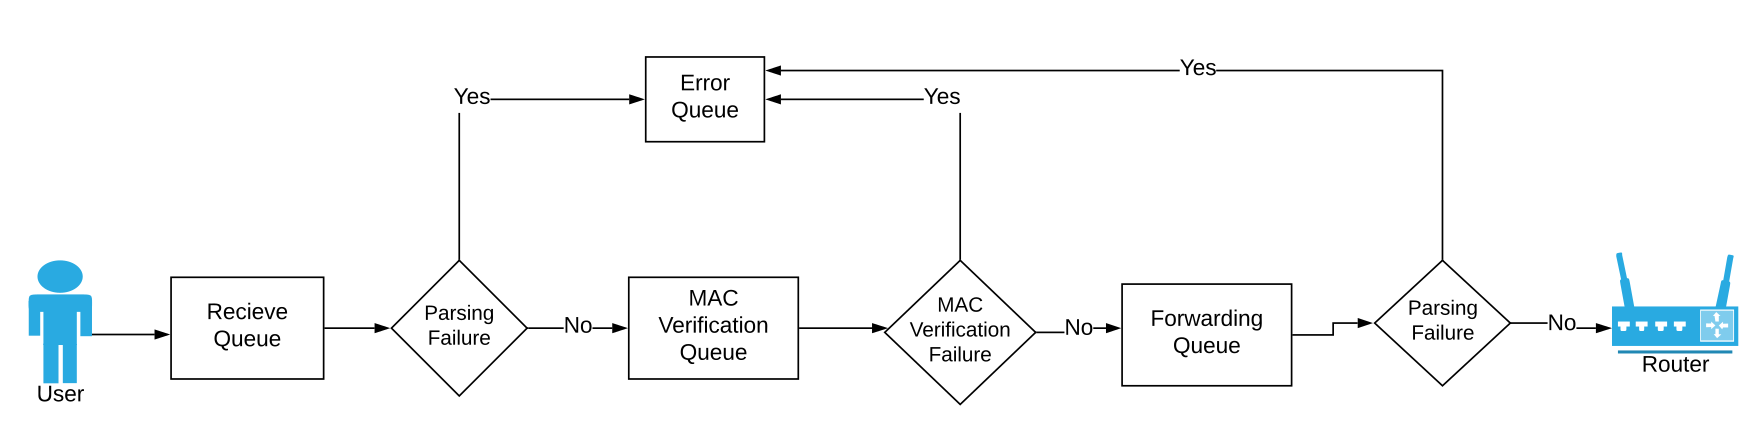
\includegraphics[scale=0.3]{Figures/svc.png}
\decoRule
\caption[APNA Service Outgoing Packet]{Outgoing Packet Processing by APNA Service}
\label{fig:perf_ephid}
\end{figure}

\subsection{Processing Incoming Packet by APNA Service}
\begin{figure}[th!!]
\centering
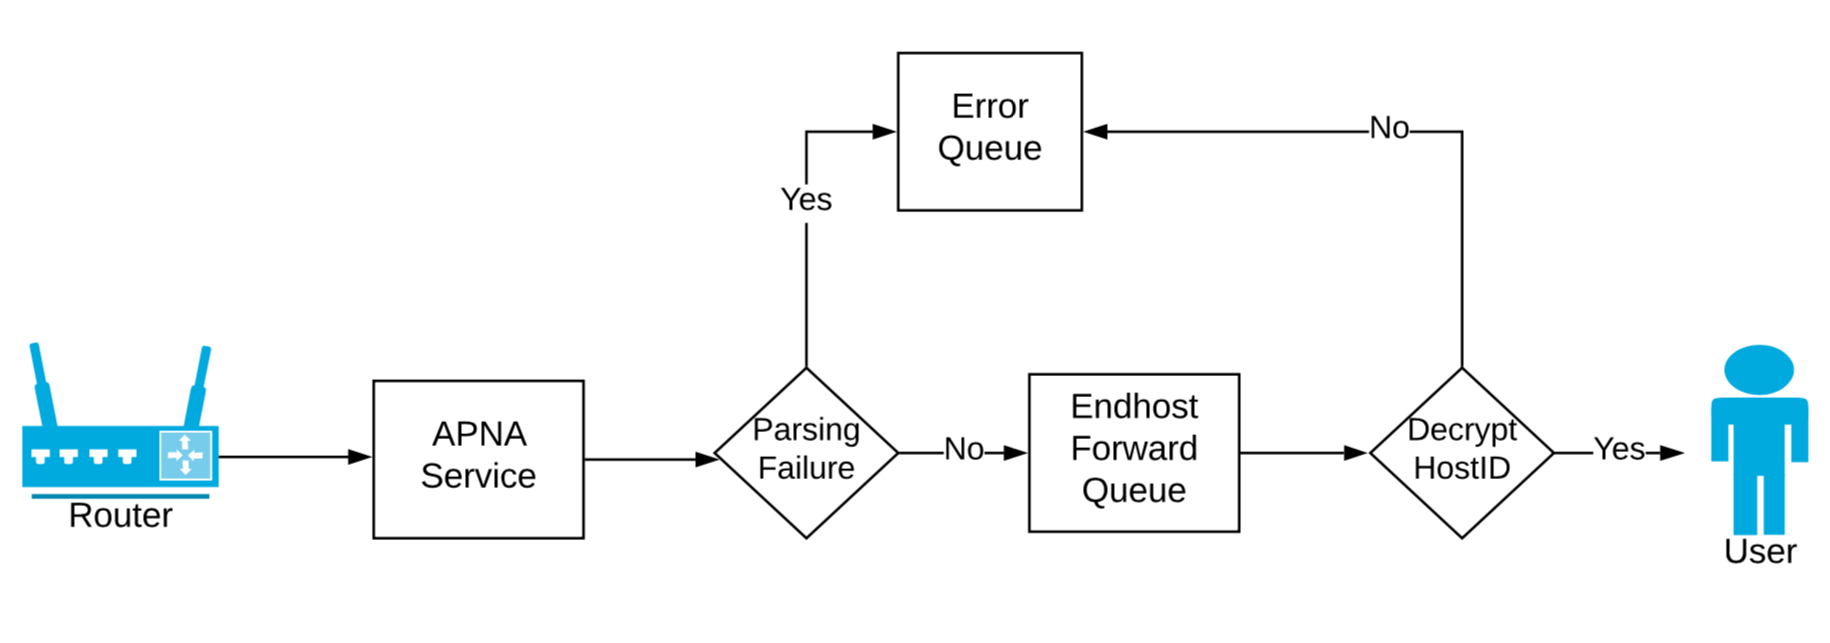
\includegraphics[scale=0.24]{Figures/svc_out.png}
\decoRule
\caption[APNA Service Incoming Packet]{Incoming Packet Processing by APNA Service}
\label{fig:perf_ephid}
\end{figure}

\section{Modifications in the current infrastructure}
\subsection{SNET}
There is a minor modification required in the existing snet implementation. First and foremost a new network string called "apna" needs to be introduced. Currently only one network is supported namely "udp4" but using this new network string we can modify the read and write functions to send/accept packets to/from APNA Service instead of directly forwarding it to border router or dispatcher.
\subsection{SCIOND}
SCIOND needs to be modified to resolve APNA Service Address (AP\_SVC)
\subsection{Border Router}
% Chapter Scion Lab Deployment

\chapter{SCIONLab Deployment} % Main chapter title
\label{scionlab} % For referencing the chapter elsewhere, use \ref{scionlab}

\section{SCIONLab Experimentation Environment}
SCIONLab  is an ongoing project that enables researchers to quickly and easily interface with the SCION network and perform experiments. The main idea of SCIONLab is that participants join the SCION network environment with their own computation resources and set up their own ASes, which get connected to the actual SCION network. The new ASes will actively participate in routing inside the SCION network. Consequently, SCIONLab enables realistic experimentation with the unique properties of SCION.

A researcher becomes a SCIONLab user by creating an account via the SCIONLab Coordination Service, creates ASes in her research institution, either on the dedicated hosts or inside virtual machines, and connects these ASes to SCIONLab ASes, which are a subset of SCION ASes with the capability to accept connections from SCIONLab users. The user can then start sending and receiving packets through the SCION network.

The operation of SCIONLab leverages the existing mechanisms and the framework developed for SCION's deployment, such as the Local Management Service, the SCIONLab Coordination Service, and Ansible. Moreover, SCIONLab also aims at hosting test versions of SCION, with new and experimental features like APNA, and also to enable SCIONLab users to connect to one another. 
% Chapter Performance Evaluation

\chapter{Performance Evaluation} % Main chapter title

\label{performance} % For referencing the chapter elsewhere, use \ref{performance}

% Chapter Conclusion

\chapter{Conclusion} % Main chapter title

\label{conclusion} 

%----------------------------------------------------------------------------------------
%	THESIS CONTENT - APPENDICES
%----------------------------------------------------------------------------------------

\appendix % Cue to tell LaTeX that the following "chapters" are Appendices

% Include the appendices of the thesis as separate files from the Appendices folder
% Uncomment the lines as you write the Appendices

% Appendix A

\chapter{Frequently Asked Questions} % Main appendix title

\label{AppendixA} % For referencing this appendix elsewhere, use \ref{AppendixA}

\section{How do I change the colors of links?}

The color of links can be changed to your liking using:

{\small\verb!\hypersetup{urlcolor=red}!}, or

{\small\verb!\hypersetup{citecolor=green}!}, or

{\small\verb!\hypersetup{allcolor=blue}!}.

\noindent If you want to completely hide the links, you can use:

{\small\verb!\hypersetup{allcolors=.}!}, or even better: 

{\small\verb!\hypersetup{hidelinks}!}.

\noindent If you want to have obvious links in the PDF but not the printed text, use:

{\small\verb!\hypersetup{colorlinks=false}!}.

%\include{Appendices/AppendixB}
%\include{Appendices/AppendixC}

%----------------------------------------------------------------------------------------
%	BIBLIOGRAPHY
%----------------------------------------------------------------------------------------

\printbibliography[heading=bibintoc]

%----------------------------------------------------------------------------------------

\end{document}  
